

\StartOf{Lecture 8}

\Today{(1) OFDM and Multicarrier Modulation, (2) Probability in Digital Comms}

\announcements{
\begin{itemize}
  \item For today: Rice 5.5 and 4.1--4.3.  
  \item For Mon: Kay book reading (Canvas). Note that we meet as normal on Feb 17.
  \item HW 3 due today; Proj 2 due Mon. 
  \item HW 4 posted, due Feb 19.  
\end{itemize}
}

\section{Orthogonal Frequency Division Multiplexing (OFDM)}

This is section 5.5 in the Rice book.

In FSK, we use a single basis function at each of different
frequencies.  In QAM, we use two basis functions at the same
frequency.  \emph{Multicarrier modulation} is the combination:
\begin{eqnarray}
 \phi_{0,c}(t) &=& \sqrt{\frac{2}{T_{s}}} p(t) \cos(\omega_0 t)
 \nnn
 \phi_{0,s}(t) &=& -\sqrt{\frac{2}{T_{s}}} p(t) \sin(\omega_0 t)
 \nnn
 \phi_{1,c}(t) &=& \sqrt{\frac{2}{T_{s}}} p(t) \cos(\omega_0 t + 2\pi \Delta f t)
 \nnn
 \phi_{1,s}(t) &=& -\sqrt{\frac{2}{T_{s}}} p(t) \sin(\omega_0 t + 2\pi \Delta f t)
 \nnn
  &\vdots & \nonumber \\
 \phi_{M-1,c}(t) &=& \sqrt{\frac{2}{T_{s}}} p(t) \cos(\omega_0 t + 2\pi (M-1)\Delta f t)
 \nnn
 \phi_{M-1,s}(t) &=& -\sqrt{\frac{2}{T_{s}}} p(t) \sin(\omega_0 t + 2\pi (M-1)\Delta f t)
 \nn
\end{eqnarray}
where $\Delta f = \frac{1}{2T_{s}}$.  In OFDM, we call the two waveforms (sine and cosine) at one frequency a ``subcarrier''.  Multi-carrier modulation is a general type of modulation, of which \emph{orthogonal frequency division multiplexing} (OFDM) is a specific version which uses the NRZ (rectanguar) pulse, non-zero only between 0 and $T_s$.  OFDM is thus represented as:
\begin{eqnarray}
 \phi_{0,c}(t) &=& \pdfarray{\sqrt{\frac{2}{T_{s}}} \cos(\omega_0 t)}{0 \le t \le T_{s}}
 \nnn
 \phi_{0,s}(t) &=& \pdfarray{-\sqrt{\frac{2}{T_{s}}} \sin(\omega_0 t)}{0 \le t \le T_{s}}
 \nnn
 \phi_{1,c}(t) &=& \pdfarray{\sqrt{\frac{2}{T_{s}}} \cos(\omega_0 t + 2\pi \Delta f t)}{0 \le t \le T_{s}}
 \nnn
 \phi_{1,s}(t) &=& \pdfarray{-\sqrt{\frac{2}{T_{s}}} \sin(\omega_0 t + 2\pi \Delta f t)}{0 \le t \le T_{s}}
 \nnn
  &\vdots & \nonumber \\
 \phi_{M-1,c}(t) &=& \pdfarray{\sqrt{\frac{2}{T_{s}}} \cos(\omega_0 t + 2\pi (M-1)\Delta f t)}{0 \le t \le T_{s}}
 \nnn
 \phi_{M-1,s}(t) &=& \pdfarray{-\sqrt{\frac{2}{T_{s}}} \sin(\omega_0 t + 2\pi (M-1)\Delta f t)}{0 \le t \le T_{s}}
 \nn
\end{eqnarray}
where again $\Delta f = \frac{1}{2T_{s}}$. 

These waveforms, for multicarrier modulation and for OFDM in particular, are all mutually orthogonal, as you will show in your homework 4.  We can transmit much more information than possible in
$M$-ary FSK.  (Note we have $2M$ basis functions here in the same bandwidth as M-ary FSK!)


The signal on subchannel $k$ for OFDM might be represented as:
\[
  x_k(t) = \sqrt{\frac{2}{T_{s}}} \left[ a_{k,I}(t) \cos(\omega_0 t  + 2\pi f_k t) - a_{k,Q}(t) \sin(\omega_0 t + 2\pi f_k t) \right]
\]
On the $k$th channel, the signal could be described as some kind of QAM or PSK modulation. Regardless, over all channels, the modulation is called OFDM.  The OFDM  signal of the sum of all $K$ signals might then be represented as
\begin{eqnarray}
  x(t) &=& \sqrt{\frac{2}{T_{s}}} \mR \left\{ \sum_{k=1}^K (a_{k,I}(t) + j a_{k,Q}(t))  e^{j(\omega_0 + 2\pi k \Delta f )t}  \right\} \nonumber \\
  x(t) &=& \sqrt{\frac{2}{T_{s}}} \mR \left\{ e^{j\omega_0 t} \sum_{k=1}^K A_{k}(t)  e^{j2\pi k \Delta f t}  \right\}
\end{eqnarray}
where $A_{k}(t) = a_{k,I}(t) + j a_{k,Q}(t)$. Does this look like an
inverse discrete Fourier transform? If yes, than you can see why it
might be possible to use an IFFT and FFT to generate the transmitted signal.

\begin{enumerate}
  \item FFT implementation:  There is a particular implementation of
  the transmitter and receiver that use FFT/IFFT operations.  This
  avoids having $K$ independent transmitter chains and receiver
  chains.  The FFT implementation (and the speed and ease of implementation of the FFT in hardware) is why OFDM
  is popular.
\end{enumerate}


Since the $K$ carriers are orthogonal, the signal is like $K$-ary
FSK. But, rather than transmitting on one of the $K$ carriers at a
given time (like FSK) we transmit information in parallel on all $K$
channels simultaneously.  An example state space diagram for $K=3$
and PAM on each channel is shown in Figure
\ref{F:OFDM-state-space-diagram}.

\begin{figure}[htbp]
  \centerline{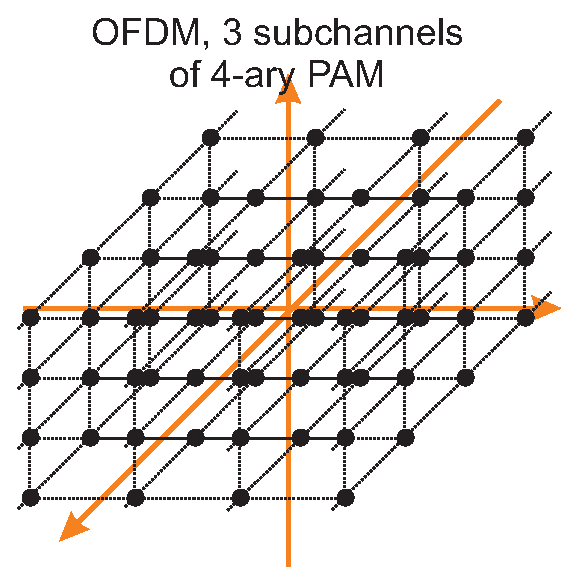
\includegraphics[width=0.45\textwidth]{../images/OFDM-K3-4PAM-signalSpaceDiagram.eps} }
  \caption{Signal space diagram for $K=3$ subchannel OFDM with 4-PAM on each channel.}
  \label{F:OFDM-state-space-diagram}
\end{figure}

\Example{802.11a}  IEEE 802.11a uses OFDM with 52 subcarriers.  Four of the subcarriers are reserved for pilot tones, so effectively 48 subcarriers are used for data.  Each data subcarrier can be modulated in different ways.  One example is to use 16 square QAM on each subcarrier (which is 4 bits per symbol per subcarrier).  The symbol rate in 802.11a is 250k/sec.  Thus the bit rate is
\[
   250\times 10^3 \frac{\mbox{OFDM symbols}}{\mbox{sec}} 48 \frac{\mbox{subcarriers}}{\mbox{OFDM symbol}} 4 \frac{\mbox{coded bits}}{\mbox{subcarrier}} = 48 \frac{\mbox{Mbits}}{\mbox{sec}}
\]



\section{Probability in Digital Communications}

Question: What is random about digital communications signals?  Why do we need probabilistic analysis tools in the design of digital communications systems?

\Solution{
Here are some of my ideas, but of course there are others:
\begin{enumerate}
    \item The data being sent
    \item Additive noise
    \item Interference from competing systems
    \item Multipath fading
    \item Doppler
    \item Transmit signal imperfections
    \item The timing of when a packet starts
    \item Transmit power
    \item Whether a receiver is awake or in sleep state at any time
    \item Frequency offset
\end{enumerate}

}

In general, random variables are (typically) unknown.  The use of probability theory and analysis is to allow us to quantify what can be known about those random systems, and to use that in engineering design of those systems.


\subsection{Distributions}

Probability distributions give us a tool to quantify how likely particular a range of values is, or even a particular value is, of a random variable.  

\vspace{0.15in}\noindent For two random variables $X_1$ and $X_2$,
\begin{itemize}
  \item Joint CDF: $F_{X_1, X_2}(x_1, x_2) = \PR{\{X_1 \le x_1\}
    \cap \{X_2 \le x_2\}}$  It is the probability that both events
    happen simultaneously.
  \item Joint pmf: $p_{X_1, X_2}(x_1, x_2) = \PR{\{X_1 = x_1\}
    \cap \{X_2 = x_2\}}$  It is the probability that both events
    happen simultaneously.
  \item Joint pdf: $f_{X_1, X_2}(x_1, x_2) = \dtwodd{x_1}{x_2} F_{X_1, X_2}(x_1, x_2)$
\end{itemize}
The (pdf / pmf) (integrates / sums) to one, and is non-negative.  The CDF is non-negative and non-decreasing, with 
$\lim_{x_i\rightarrow.-\infty} F_{X_1, X_2}(x_1, x_2) = 0$ and $\lim_{x_1,x_2 \rightarrow.+\infty} F_{X_1, X_2}(x_1, x_2) = 1$.



\vspace{0.15in}\noindent To find the probability of an event, you
integrate.  For example, for event $B \in S$,
\begin{itemize}
  \item Discrete case: $\PR{B} = \sum \sum_{(X_1,X_2) \in B} p_{X_1, X_2}(x_1, x_2)$
  \item Continuous Case: $\PR{B} = \int \int_{(x_1,x_2) \in B} f_{X_1, X_2}(x_1,  x_2) dx_1 dx_2$
\end{itemize}

\vspace{0.15in}\noindent The marginal distributions are:
\begin{itemize}
  \item Marginal pmf: $p_{X_2}(x_2) = \sum_{x_1 \in S_{X_1}} p_{X_1, X_2}(x_1, x_2)$
  \item Marginal pdf: $f_{X_2}(x_2) = \int_{x_1 \in S_{X_1}} f_{X_1, X_2}(x_1,
  x_2) dx_1$
\end{itemize}

\vspace{0.15in}\noindent Two random variables $X_1$ and $X_2$ are
independent iff for all $x_1$ and $x_2$,
\begin{itemize}
  \item $p_{X_1, X_2}(x_1, x_2) = p_{X_1}(x_1) p_{X_2}(x_2)$
  \item $f_{X_1, X_2}(x_1, x_2) = f_{X_2}(x_2) f_{X_1}(x_1)$
\end{itemize}

\subsection{Random Vectors}

\Definition{Random Vector}{A random vector (R.V.) is a list of
multiple random variables $X_1, X_2, \ldots, X_n$,
\[
\mbX = [X_1, X_2, \ldots, X_n]^T
\]
}

Here are the Models of R.V.s:
\begin{enumerate}
  \item The CDF of R.V. $\mbX$ is $F_{\mbX}(\mbx) = F_{X_1, \ldots,
    X_n}(x_1, \ldots, x_n)$ $= \PR{X_1 \le x_1, \ldots, X_n \le x_n}$.
  \item The pmf of a discrete R.V. $\mbX$ is $p_{\mbX}(\mbx) $ $= p_{X_1, \ldots,
    X_n}(x_1, \ldots, x_n) $  $= \PR{X_1 = x_1, \ldots, X_n = x_n}$.
  \item The pdf of a continuous R.V. $\mbX$ is $f_{\mbX}(\mbx) $ $= f_{X_1, \ldots,
    X_n}(x_1, \ldots, x_n) $ $= \tfrac{\partial^n}{\partial x_1 \cdots \partial x_n} F_{\mbX}(\mbx)$.
\end{enumerate}

\subsection{Conditional Distributions}

\vspace{0.15in}\noindent Given event $B \in S$ which has $\PR{B}>0$,
the joint probability conditioned on event $B$ is
\begin{itemize}
  \item Discrete case:
    \[ p_{X_1, X_2 | B}(x_1, x_2) = \pdfarray{\frac{p_{X_1, X_2}(x_1, x_2)}{ \PR{B}}}{(X_1, X_2) \in B}
    \]
  \item Continuous Case:
    \[ f_{X_1, X_2 | B}(x_1, x_2) = \pdfarray{\frac{f_{X_1, X_2}(x_1, x_2)}{ \PR{B}}}{(X_1, X_2) \in B}
    \]
\end{itemize}

\vspace{0.15in}\noindent Given r.v.s $X_1$ and $X_2$,
\begin{itemize}
  \item Discrete case.  The conditional pmf of $X_1$ given $X_2=x_2$, where $p_{X_2}(x_2) > 0$, is
    \[ p_{X_1| X_2 }(x_1| x_2) = p_{X_1, X_2}(x_1 , x_2) / p_{X_2}(x_2)
    \]
  \item Continuous Case:  The conditional pdf of $X_1$ given
  $X_2=x_2$, where $f_{X_2}(x_2) > 0$, is
    \[ f_{X_1| X_2 }(x_1| x_2) = f_{X_1, X_2}(x_1, x_2) / f_{X_2}(x_2)
    \]
\end{itemize}

\Definition{Bayes' Law}{Bayes' Law is a reformulation of he
definition of the marginal pdf.  It is written either as:
  \[
      f_{X_1,X_2}(x_1,x_2) = f_{X_2|X_1}(x_2|x_1) f_{X_1}(x_1)
  \]
  or
  \[
      f_{X_1|X_2}(x_1|x_2) = \frac{f_{X_2|X_1}(x_2|x_1)
      f_{X_1}(x_1)}{f_{X_2}(x_2)}
  \]
}

\subsection{Simulation of Digital Communication Systems}

A simulation of a digital communication system is often used to
estimate a bit error rate.  Each bit can either be demodulated
without error, or with error.  Thus the simulation of one bit is a
Bernoulli trial.  This trial $E_i$ is in error ($E_1=1$) with
probability $p_e$ (the true bit error rate) and correct ($E_i=0$)
with probability $1-p_e$.  What type of random variable is $E_i$?

Simulations run many bits, say $N$ bits through a model of the
communication system, and count the number of bits that are in
error.  Let $S = \sum_{i=1}^N E_i$, and assume that $\{E_i\}$ are
independent and identically distributed (i.i.d.).
\begin{enumerate}
  \item What type of random variable is $S$?
  \item What is the pmf of $S$?
  \item What is the mean and variance of $S$?
\end{enumerate}

\Solution{$E_i$ is called a Bernoulli r.v.~and $S$ is called a Binomial r.v., with pmf
\[
  p_S(s) = {N \choose s} p_e^s (1-p_e)^{N-s}
\]
The mean of $S$ is the the same as the mean of the sum of $\{E_i\}$,
\begin{eqnarray}
  \E{S}{S} &=& \E{\{E_i\}}{\sum_{i=1}^N E_i} = \sum_{i=1}^N  \E{E_i}{E_i} \nnn
   &=& \sum_{i=1}^N   \left[ (1-p)\cdot 0 + p \cdot 1\right] = Np \nn
\end{eqnarray}
We can find the variance of $S$ the same way:
\begin{eqnarray}
  \Var{S}{S} &=& \Var{\{E_i\}}{\sum_{i=1}^N E_i} = \sum_{i=1}^N  \Var{E_i}{E_i} \nnn
   &=& \sum_{i=1}^N   \left[ (1-p)\cdot (0-p)^2 + p \cdot (1-p)^2\right]
   \nnn
   &=& \sum_{i=1}^N   \left[ (1-p)p^2 + (1-p)(p-p^2)\right] 
   \nnn
   &=&   Np(1-p)
   \nn
\end{eqnarray}
}

We may also be interested knowing how many bits to run in order to
get an estimate of the bit error rate.  For example, if we run a
simulation and get zero bit errors, we won't have a very good idea
of the bit error rate.  Let $T_1$ be the time (number of bits) up to and including the first error.
\begin{enumerate}
  \item What type of random variable is $T_1$?
  \item What is the pmf of $T_1$?
  \item What is the mean of $T_1$?
\end{enumerate}

\Solution{$T_1$ is a Geometric r.v. with pmf
\[
  p_{T_1}(t) = (1-p_e)^{t-1} p_e
\]
The mean of $T_1$ is
\[
  \E{}{T_1} = \frac{1}{p_e}
\]
Note the variance of $T_1$ is $\Var{}{T_1} = (1-p_e)/p_e^2$, so the
standard deviation for very low $p_e$ is almost the same as the
expected value.}

So, even if we run an experiment until the first bit error, our
estimate of $p_e$ will have relatively high variance.

% \subsection{Mixed Discrete and Continuous Joint Variables}
% 
% This was not covered in ECE 5510, although it was in the Yates \&
% Goodman textbook.  We'll often have $X_1$ discrete and $X_2$
% continuous.
% 
% \Example{Digital communication system in noise} Let $X_1$ is the
% transmitted signal voltage, and $X_2$ is the received signal
% voltage, which is modeled as
% \[
% X_2 = a X_1 + N
% \]
% where $N$ is a continuous-valued random variable representing the
% additive noise of the channel, and $a$ is a constant which
% represents the attenuation of the channel.  In a digital system,
% $X_1$ may take a discrete set of values, \eg, $\{ 1.5, 0.5, -0.5,
% -1.5\}$.  But the noise $N$ may be continuous, \eg, Gaussian with
% mean $\mu$ and variance $\sigma^2$.  As long as $\sigma^2>0$, then
% $X_2$ will be continuous-valued.
% 
% \vspace{0.15in}\noindent \textbf{Work-around}:  We will sometimes
% use a pdf for a discrete random variable.  For instance, if
% \[
%   p_{X_1}(x_1) = \pdfarrays{0.6}{x_1 = 0}{0.4}{x_1=1}
% \]
% then we would write a pdf with the probabilities as amplitudes of a
% dirac delta function centered at the value that has that
% probability,
% \[
%   f_{X_1}(x_1) = 0.6\delta(x_1) + 0.4\delta(x_1-1)
% \]
% This pdf has integral 1, and non-negative values for all $x_1$.  Any
% probability integral will return the proper value.  For example, the
% probability that $-0.5 < x_1 < 0.5$ would be an integral that would
% return 0.6.
% 
% \Example{Joint distribution of $X_1, X_2$} Consider the channel
% model $X_2 = X_1 + N$, and
% \[
%  f_N(n) = \frac{1}{\sqrt{2\pi \sigma^2}} e^{-n^2/(2\sigma^2)}
% \]
% where $\sigma^2$ is some known variance, and the r.v. $X_1$ is
% independent of $N$ with
% \[
%   p_{X_1}(x_1) = \pdfarrays{0.5}{x_1 = 0}{0.5}{x_1=1}.
% \]
% \begin{enumerate}
%   \item What is the pdf of $X_2$?
%   \item What is the joint p.d.f.~of $(X_1, X_2)$ ?
% \end{enumerate}
% 
% \Solution{
% \begin{enumerate}
%   \item When two independent r.v.s are added, the pdf of the sum is the
%     \emph{convolution} of the pdfs of the inputs.  Writing
%     \[
%       f_{X_1}(x_1) = 0.5 \delta(x_1) + 0.5 \delta(x_1-1)
%     \]
%     we convolve this with $f_N(n)$ above, to get
%     \begin{eqnarray}
%       f_{X_2}(x_2) &=& 0.5 f_N(x_2) + 0.5f_N(x_2-1) \nonumber \\
%       f_{X_2}(x_2) &=& \frac{1}{2\sqrt{2\pi \sigma^2}} \left[
%           e^{-x_2^2/(2\sigma^2)} + e^{-(x_2-1)^2/(2\sigma^2)}
%         \right] \nonumber
%     \end{eqnarray}
%   \item What is the joint p.d.f.~of $(X_1, X_2)$ ?
%     Since $X_1$ and $X_2$ are NOT independent, we cannot simply multiply
%     the marginal pdfs together.  It is necessary to use Bayes' Law.
%     \[
%       f_{X_1,X_2}(x_1,x_2) = f_{X_2|X_1}(x_2|x_1) f_{X_1}(x_1)
%     \]
%     Given a value of $X_1$ (either 0 or 1) we can write down the pdf
%     of $X_2$.  So break this into two cases:
%     \begin{eqnarray}
%        f_{X_1,X_2}(x_1,x_2) &=& \pdfarrays{f_{X_2|X_1}(x_2|0)
%          f_{X_1}(0)}{x_1 = 0}{f_{X_2|X_1}(x_2|1)
%          f_{X_1}(1)}{x_1 = 1} \nonumber \\
%        f_{X_1,X_2}(x_1,x_2) &=& \pdfarrays{ 0.5 f_N(x_2)}{x_1 = 0}{0.5f_N(x_2-1)}{x_1 = 1} \nonumber \\
%        f_{X_1,X_2}(x_1,x_2) &=& 0.5 f_N(x_2) \delta(x_1)  + \nnn
%                             & & 0.5 f_N(x_2-1) \delta(x_1 - 1) \nonumber
%     \end{eqnarray}
%     These last two lines are completely equivalent.  Use
%     whichever seems more convenient for you.  See Figure
%     \ref{F:MixedPdfExample}.
% \end{enumerate}
% }
% \begin{figure}[htb]
%   \centerline{\psfig{figure=plotMixedPdfExample.eps,width=3in}}
%   \caption{Joint pdf of $X_1$ and $X_2$, the input and output (respectively) of the example additive noise communication system, when $\sigma=1$.}
%   \label{F:MixedPdfExample}
% \end{figure}

\subsection{Expectation}

\Definition{Expected Value (Joint)}{ The expected value of a
function $g(X_1, X_2)$ of random variables $X_1$ and $X_2$ is given
by,
\begin{enumerate}
  \item Discrete: $\E{}{g(X_1, X_2)} =
     \sum_{X_1 \in S_{X_1}} \sum_{X_2 \in S_{X_2}} g(X_1, X_2) p_{X_1, X_2}(x_1, x_2)$
  \item Continuous: $\E{}{g(X_1, X_2)} =
     \int_{X_1 \in S_{X_1}} \int_{X_2 \in S_{X_2}} g(X_1, X_2) f_{X_1, X_2}(x_1, x_2)$
\end{enumerate}}

Typical functions $g(X_1, X_2)$  are:
\begin{itemize}
  \item Mean of $X_1$ or $X_2$:  $g(X_1, X_2) = X_1$ or $g(X_1, X_2) =
    X_2$ will result in the means $\mu_{X_1}$ and $\mu_{X_2}$.
  \item Variance (or 2nd central moment) of $X_1$ or $X_2$:  $g(X_1, X_2) = (X_1-\mu_{X_1})^2$ or $g(X_1, X_2) =
    (X_2-\mu_{X_2})^2$.  Often denoted $\sigma_{X_1}^2$ and
    $\sigma_{X_2}^2$.
  \item Covariance of $X_1$ and $X_2$: $g(X_1, X_2) =
    (X_1-\mu_{X_1})(X_2-\mu_{X_2})$.
  \item Expected value of the product of $X_1$ and $X_2$, also called the `correlation' of $X_1$ and $X_2$: $g(X_1, X_2) =
    X_1 X_2$.
\end{itemize}

% Stopped here, S09 Lecture 6.

\subsection{Gaussian Random Variables}

For a single Gaussian r.v. $X$ with mean $\mu_X$ and variance
$\sigma_X^2$, we have the pdf,
\[
  f_X(x) = \frac{1}{\sqrt{2\pi \sigma_X^2}} e^{-\frac{(x-\mu_X)^2}{2\sigma^2}}
\]
Consider $Y$ to be Gaussian  with mean 0 and variance 1.  The distribution of $Y$ is also called \emph{standard normal} in the statistics community without any sense of shame for the redundancy of the two words.  Regardless, we define a new symbol for the CDF of standard normal r.v.\ $Y$: 
CDF of $Y$ is denoted as $F_Y(y) = \PR{Y \le y} = \Phi(y)$.  So, for
$X$, which has non-zero mean and non-unit-variance, we can write its
CDF as
\[
  F_X(x) = \PR{X\le x} = \Phi \left( \frac{x-\mu_X}{\sigma_X} \right)
\]
You can prove this by showing that the event $X \le x$ is the same
as the event
\[
  \frac{X-\mu_X}{\sigma_X} \le \frac{x-\mu_X}{\sigma_X}
\]
Since the left-hand side is a unit-variance, zero mean Gaussian
random variable, we can write the probability of this event using
the unit-variance, zero mean Gaussian CDF.

\subsubsection{Complementary CDF}
The probability that a unit-variance, zero mean Gaussian r.v. $X$ exceeds some value $x$ is one minus the
CDF, that is, $1-\Phi(x)$.  This is so common in digital communications, it is given its
own name, $Q(x)$,
\[
  Q(x) = \PR{X >  x} = 1 - \Phi \left( x \right)
\]
What is $Q(x)$ in integral form?
\[
  Q(x) = \int_x^\infty \frac{1}{\sqrt{2\pi}} e^{-w^2/2} dw
\]
For an Gaussian r.v. $X$ with variance $\sigma_X^2$,
\[
  \PR{X >  x} = Q\left( \frac{x-\mu_X}{\sigma_X} \right)  = 1 - \Phi \left( \frac{x-\mu_X}{\sigma_X} \right)
\]

\subsubsection{Error Function}

In math, in some texts, and in Matlab, the $Q(x)$ function is not
used.  Instead, there is a function called $\erf(x)$
\[
  \erf(x) \triangleq \frac{2}{\sqrt{\pi}} \int_0^x e^{-t^2} dt
\]


\Example{Relationship between $Q(\cdot)$ and $\erf(\cdot)$}  What is
the functional relationship between $Q(\cdot)$ and $\erf(\cdot)$?

\Solution{ Substituting $t=u/\sqrt{2}$ (and thus $dt =
  du/\sqrt{2}$),
  \begin{eqnarray}
    \erf(x) &\triangleq& \frac{2}{\sqrt{2\pi}} \int_0^{\sqrt{2}x} e^{-u^2/2}
    du \nonumber \\
            &=& 2 \int_0^{\sqrt{2}x} \frac{1}{\sqrt{2\pi}} e^{-u^2/2}
    du \nonumber \\
            &=& 2  \left( \Phi(\sqrt{2}x) - \frac{1}{2} \right) \nonumber
  \end{eqnarray}
  Equivalently, we can write $\Phi(\cdot)$ in terms of the
  $\erf(\cdot)$ function,
  \[
    \Phi(\sqrt{2}x) = \frac{1}{2} \erf(x) + \frac{1}{2}
  \]
  Finally  let $y=\sqrt{2}x$, so that
  \[
    \Phi(y) = \frac{1}{2} \erf\left(\frac{y}{\sqrt{2}}\right) + \frac{1}{2}
  \]
  Or in terms of $Q(\cdot)$,
  \begin{equation}\label{E:QInTermsOfErf}
    Q(y) = 1-\Phi(y) = \frac{1}{2} - \frac{1}{2} \erf\left(\frac{y}{\sqrt{2}}\right)
  \end{equation}
}
You should go to Matlab and create a function Q(y) which implements:
\begin{verbatim}
    function rval = Q(y)
    rval = 0.5.*erfc(y./sqrt(2));
\end{verbatim}
In Python there is an erfc function in both math and scipy.special packages.

 \Example{Probability of Error in Binary Example} As in the
previous example, we have a model system in which the receiver sees
$X_2 = X_1 + N$.  Here, $X_1 \in \{0,1\}$ with equal probabilities
and $N$ is independent of $X_1$ and zero-mean Gaussian with variance
$1/4$. The receiver decides as follows:
\begin{itemize}
  \item If $X_2 \le 1/3$, then decide that the transmitter sent a `0'.
  \item If $X_2 > 1/3$, then decide that the transmitter sent a `1'.
\end{itemize}
\begin{enumerate}
  \item Given that $X_1=1$, what is the probability that the receiver decides that a `0' was sent?
  \item Given that $X_1=0$, what is the probability that the receiver decides that a `1' was sent?
\end{enumerate}

\Solution{
  \begin{enumerate}
    \item Given that $X_1=1$, since $X_2 = X_1 + N$, it is clear that $X_2$ is also a Gaussian r.v. with mean 1 and variance 1/4.
          Then the probability that the receiver decides `0' is the
          probability that $X_2 \le 1/3$,
          \begin{eqnarray}
            \PR{error | X_1=1} &=& \PR{X_2 \le 1/3}
            = \PR{\frac{X_2-1}{\sqrt{1/4}} \le \frac{1/3 - 1}{\sqrt{1/4}}}
                \nonumber \\
            &=& 1 - Q \left( (-2/3)/(1/2) \right) 
                = 1- Q(-4/3)
                \nonumber
          \end{eqnarray}
    \item Given that $X_1=0$, the probability that the receiver decides `1' is the
          probability that $X_2 > 1/3$,
          \begin{eqnarray}
            \PR{error | X_1=0} &=& \PR{X_2 > 1/3}
            = \PR{\frac{X_2}{\sqrt{1/4}} > \frac{1/3}{\sqrt{1/4}}}
                \nonumber \\
            &=& Q \left( (1/3)/(1/2) \right) 
            = Q(2/3)
                \nonumber
          \end{eqnarray}
  \end{enumerate}
}


